\documentclass[paper-main.tex]{subfiles}


\begin{document}

A continuous-wave signal may wander slowly (and randomly) in frequency over time, due to stochastic internal processes in the superfluid interior of isolated neutron stars, or variable accretion from a stellar companion for neutron stars in binaries such as LMXBs (see Ref.~\cite{SuvorovaEtAl:2017} and references therein).
Although continuous gravitational waves are nearly monochromatic, the long observing times ($\sim 1\,{\rm yr}$) mean that searches are sensitive to very small frequency drifts. \han{note}
A typical observation involves $1 \times 10^{10}$ wave cycles, and a coherent search must track the phase to better than half a cycle over the full observation. 
Here we consider the audio analog of a tone that wanders in frequency. 



A Fourier transform applied to the whole dataset (as in Section~\ref{sec:single_tone}) is not well suited to the wandering frequency case as the signal is spread across multiple frequency bins. 
In continuous-wave searches, the wandering frequency problem is solved using the Viterbi algorithm,\cite{Viterbi:1967} which can track the signal's frequency over time.
The analysis described and presented in this section is directly inspired by real continuous-wave search methods~\cite{SuvorovaEtAl:2017} yet is pitched at a level appropriate for an undergraduate laboratory setting. 
In Section~\ref{sec:realCWSearches}, we briefly review the analysis method used by LIGO and Virgo; in Section~\ref{sec:viterbi}, we describe the methods as applied in this work; and in Section~\ref{sec:wanderingResults}, we show results for recovering a wandering frequency signal using the table-top interferometer. 


\subsection{Continuous wave analysis with real data}
\label{sec:realCWSearches}


The methods used here are inspired by LIGO and Virgo continuous-wave searches. 
For further details on these methods and continuous-wave searches, we refer the reader to the references in the Supplementary Material. 


Continuous-wave searches are performed on long datasets, months to years in duration. 
The frequency of the signal can wander significantly over the observation period. 
In this context, ``significantly'' means across multiple frequency bins, where the typical width of a frequency bin is the reciprocal of the total observation time.\cite{JKS:1998,ScoX1O2Viterbi:2019}


A ``hidden Markov model'' can be used to search for continuous gravitational waves.\cite{SuvorovaEtAl:2017} 
In a Markov process, the current state depends only on the previous state (in this case the ``state'' is the frequency of the signal). 
In a hidden Markov model, the frequency state of the signal is unknown (hidden) and can undergo transitions at discrete times. 
The transitions are Markovian in that the hidden state (i.e.\ frequency) of the system at any time depends solely on its state at the previous time. 


A detection statistic relates the observed data to the hidden state and quantifies the likelihood of a signal being present in the data at each frequency and time bin.
This likelihood is also called the emission probability in gravitational-wave literature.  
In gravitational-wave data analysis, the detection statistic gives the likelihood of a signal given the antenna beam pattern of the detector, which varies as the Earth rotates and orbits the Sun.\cite{JKS:1998}
When searching for continuous waves from a neutron star in a binary (such as an LMXB), the Doppler modulation of the source also needs to be taken into account and a different detection statistic is used.\cite{SuvorovaEtAl:2017}


In continuous-wave searches, a physical model of the target informs how far the frequency of the signal can wander over time. 
This is called the transition probability matrix. 
For example, in LMXB searches, the transition matrix allows the signal frequency to (i) stay in the same frequency bin, (ii) move up a single frequency bin, or (iii) move down a frequency bin in each time step.\cite{ScoX1O2Viterbi:2019}
In supernova remnant searches, source frequency is expected to decrease over time, therefore the allowable transitions are to (i) remain in the same frequency bin, or (ii) move down one frequency bin (see the Supplementary Material for LMXB and supernova remnant search references). 


The Viterbi algorithm~\cite{Viterbi:1967} is used to find the most probable sequence of hidden frequency states given the sequence of observables.
In the next section, we describe our application of the Viterbi method and our choice of detection statistic. 




\subsection{The hidden Markov model and Viterbi algorithm}
\label{sec:viterbi}

\begin{figure}
\begin{center}
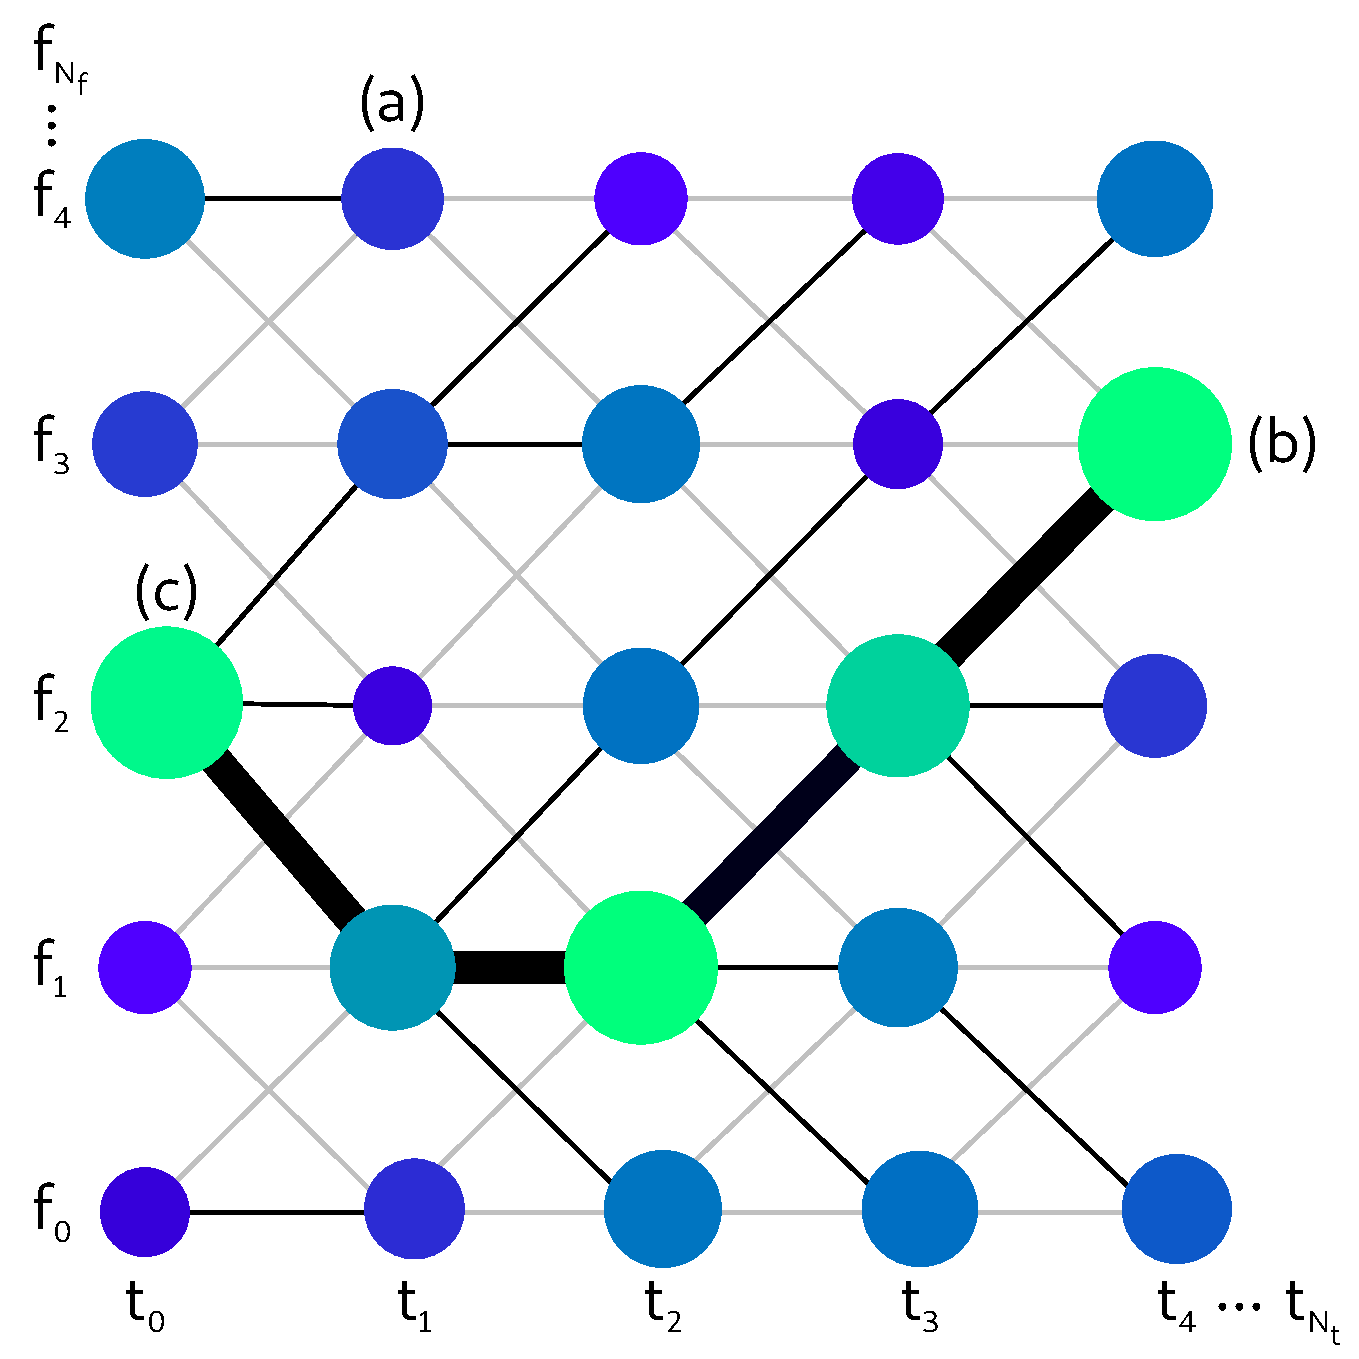
\includegraphics[width=0.48\textwidth]{figures/viterbiDiagramSizes.pdf}
\caption{\label{fig:viterbi}
Schematic diagram of the Viterbi algorithm. 
The circular nodes represent elements in a time-frequency grid, labeled $t_0$ to $t_{N_t}$ (left to right) in time and $f_0$ to $f_{N_f}$ (bottom to top) in frequency. 
The size of the nodes represents the likelihood of a signal being present in each time-frequency element. 
The small to large sizing corresponds to low to high likelihood values in arbitrary units for this schematic. 
The color gradient (online only) also represents the likelihood values where the dark blue corresponds to low likelihood and light green corresponds to high likelihood. 
The objective is to find the most probable path of a signal through the grid from left to right.
All possible paths are shown by the lines. 
The black lines show the best path to each node and the gray lines show rejected paths. 
Some routes through the grid result in dead-ends with respect to optimally reaching the other side, such as the path ending at $t_1$ marked (a).
At $t=t_{N_t}$ the algorithm chooses the terminating frequency node which has the highest value given by Eqn.~\ref{eqn:pathprobability}, marked (b). 
The Viterbi path is the path leading to this node, highlighted by the thick-black lines, from (b) to the start at (c). 
}
\end{center}
\end{figure}




First, we split the timeseries data from the interferometer into segments. 
Then, we take the discrete Fourier transform of each timeseries segment to form a grid in time and frequency (a spectrogram) with the Fourier amplitude $F(t_i,f_j)$ at frequency $f_j$ and time $t_i$, as the detection statistic (this is the emission probability).
Assuming Gaussian noise, this detection statistic maximizes the likelihood of detecting a sinusoidal signal as described in Appendix~\ref{app:sinusoid_likelihood}.
The detection statistic is normalized for convenience by dividing each value by the maximum Fourier amplitude in the grid (such that $\max_{i,j} F(t_i,f_j) = 1$).




Fig.~\ref{fig:viterbi} represents a spectrogram with $N_t$ time bins and $N_f$ frequency bins.
The circlular nodes represent the elements of the time and frequency grid, which are labelled as  
$t_i$ and $f_j$, respectively, where $i=0,1,2,\mathellipsis,N_t$ and $j=0,1,2,\mathellipsis,N_f$. 
The shading of the nodes represents the detection statistic $F(t_i,f_j)$ (the observable) at each grid point, where dark corresponds to lower values and light to higher values. 


The objective is to find the most likely path through the grid, given the observed data and any probabilistic constraints on how the frequency of the signal can wander from $t_i$ to $t_{i+1}$. 
The transition probability matrix, $A(f_k,f_m)$, describes the probability of the system transitioning from state $f_k$ at $t_i$ to a state $f_{m}$ at $t_{i+1}$. 
Here, we allow the frequency of the signal to either (i) stay in the same bin, (ii) move up by a single frequency bin, or (iii) move down by a single frequency bin at each transition. 
We assign these three transitions equal probability, i.e.\ $A(f_k,f_m)=1/3$ for $k=m+1,m,m-1$ and $A(f_k,f_m)=0$ otherwise.
All possible transitions are shown as lines in Fig.~\ref{fig:viterbi}.
The different line colors are explained below. 





Before we begin analyzing the data, we have no prior knowledge as to which frequency bin the signal starts in (i.e. the prior is flat between the minimum and maximum frequency bins).
At the first stage of the analysis, we define the probability of the system having frequency $f_j$ at the initial time $t_0$ to be equal to the (normalized) detection statistic of that state (i.e.\  ${\rm Pr}[f(t_0) = f_j] = F[t_0,f_j]$).
A specific path (which may not be optimal) is written as $f(t_0), f(t_1),\mathellipsis, f(t_n)$. 
The probability of a specific path given the data is 
\begin{eqnarray}
{\rm Pr}[ f(t_0), f(t_1),&&\mathellipsis, f(t_n) | {\rm data}] \nonumber\\
          && =F[t_n,f(t_n)] A[f(t_n),f(t_{n-1})] \nonumber \\
          && \times\mathellipsis\times A[f(t_1),f(t_0)] F[t_0,f(t_0)] \,.
\label{eqn:pathprobability}
\end{eqnarray}
The path $f^\ast(t_0),\mathellipsis,f^\ast(t_n)$ that maximises ${\rm Pr}[ f(t_0), f(t_1),\mathellipsis, f(t_n) | {\rm data}]$ is the optimal path terminating in the frequency bin $f^\ast(t_n)$. 
We note that the left-hand-side and right-hand-side of Eqn.~\ref{eqn:pathprobability} are both evaluated for a specific path and then we maximize over all such paths to find the optimal Viterbi path. 


The Viterbi algorithm provides a computationally efficient method for finding the optimal path. 
At every $t_i$ all but $N_f$ possible paths are eliminated. 
Here we describe the algorithm while referring to the schematic in Fig.~\ref{fig:viterbi}.  
The implementation used in this work is available online (see Appendix~\ref{app:code}) and we provide further information (including pseudocode) in Appendix~\ref{app:viterbi}.
\begin{enumerate}
\item Starting at time $t_1$, each $f_j$ node (circles in Fig~\ref{fig:viterbi}) can originate from three prior nodes at time $t_0$ (except for the edge cases $f_0$ and $f_{N_f}$ which only have two). 
The paths between these nodes are indicated by the lines in Fig.~\ref{fig:viterbi}. 
At each $f_j$ node, we select the path with the highest $A[f(t_0),f(t_1)] {\rm Pr}[f(t_0)]$ value as the most probable path. 
These choices are highlighted using the black lines in Fig.~\ref{fig:viterbi} while the gray lines show the rejected paths. 
For example, the most probable connection to the node labeled (a) is the one directly behind it (i.e., $f_4$). 
Therefore, this path is selected as the best path from $t_0$ to $t_1$ for $f_4$.
To allow backtracking at the end, the index of the most probable connection to a node along with the value of the best path to that node is stored, for each node.

\item Moving to time $t_2$, again we select the path which maximizes Eqn.~\ref{eqn:pathprobability} for each $f_j$. 
These paths are again shown by the solid black lines between the nodes at $t_1$ and $t_2$ in Fig.~\ref{fig:viterbi}.
Rejected paths are again shown by gray lines. 

\item Step 2 is repeated until the end of the grid ($t=t_{N_t}$) is reached with only the best paths being stored at each iteration. 

\item We have now found the most probable path to each $f_j$ at $t=t_{N_t}$ and its probability (Eqn.~\ref{eqn:pathprobability}). 
We select the terminating frequency bin $f(t_{N_t})$ with the highest probability labeled as (b) in Fig.~\ref{fig:viterbi}.

\item The final step is to find the Viterbi path (the overall best path that terminates in the frequency bin with the highest probability in step 4). 
The Viterbi path is found by backtracking along the stored best connections at each $t_i$ (see also Appendix~\ref{app:viterbi}). 
In Fig.~\ref{fig:viterbi}, it is the path ending at (b) that started at (c) highlighted by the thick-black lines.
\end{enumerate}

In continuous gravitational wave searches, the signal amplitude is expected to be small in comparison to the noise and its frequency can change unpredictably over time. % how to hyphenate ``continuous gravitational wave searches''?
The Viterbi algorithm's strength lies in its ability to track such signals through the data even in the presence of comparatively loud noise fluctuations in the time-frequency bins.
In the following section, we present the results of using the Viterbi algorithm with the table-top interferometer data. 







\subsection{Wandering frequency signal results}
\label{sec:wanderingResults}

\begin{figure*}
	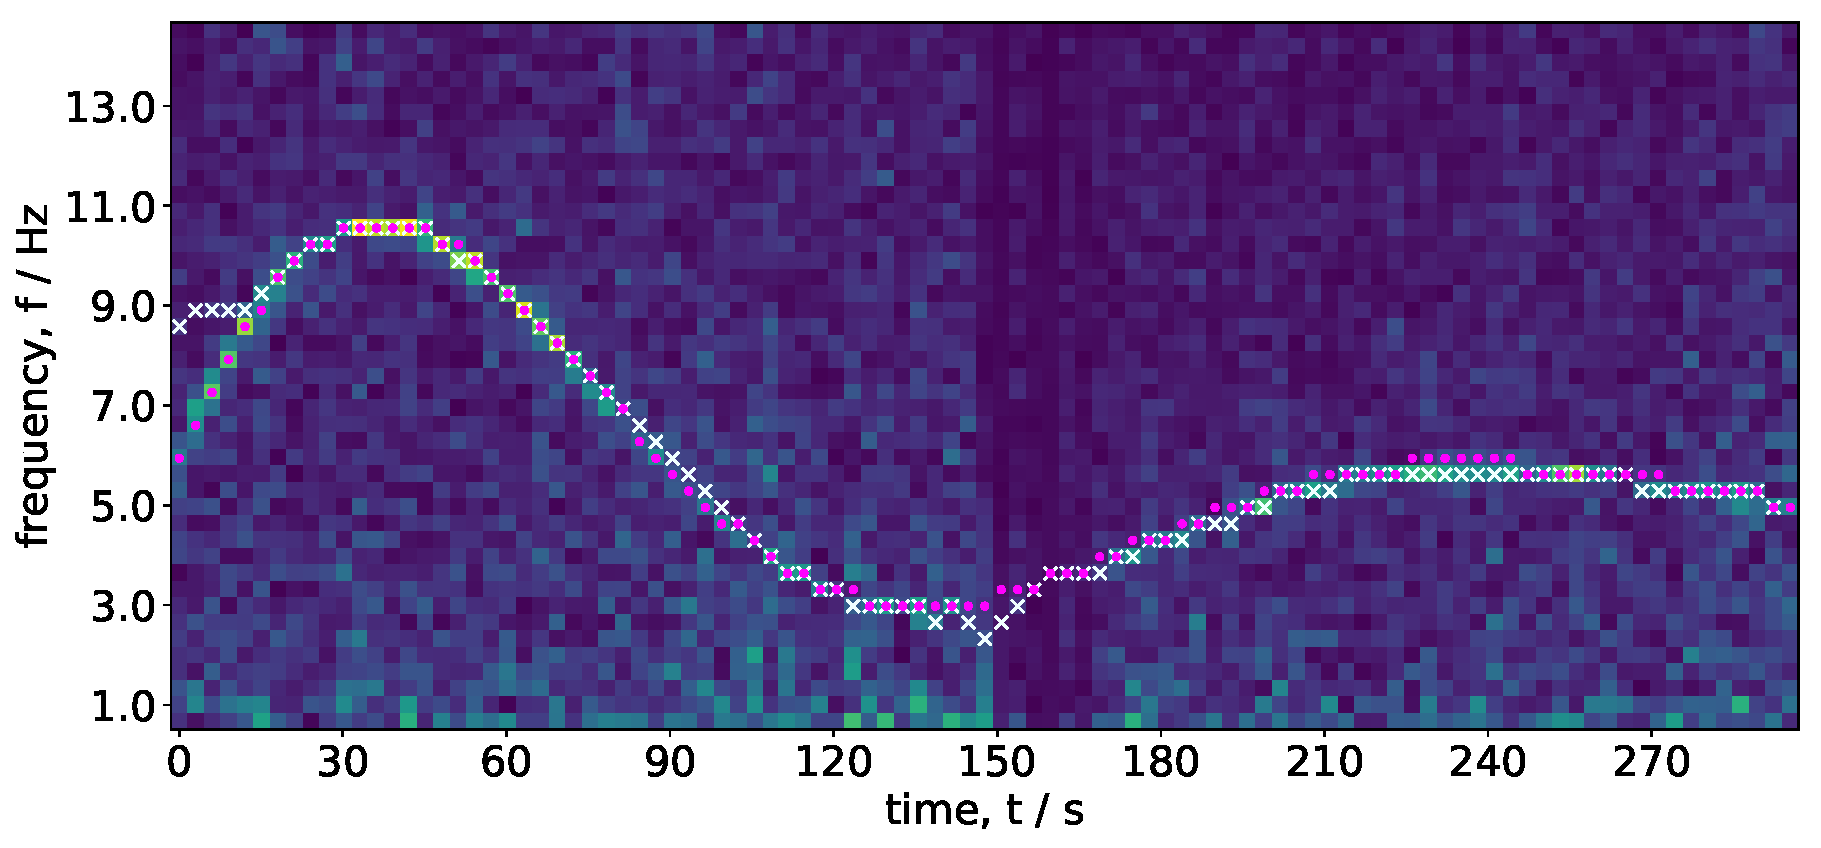
\includegraphics[width=\textwidth]{figures/expt_overlay_2_viterbi_test_webcam.pdf}
	\caption{\label{fig:viterbi_overlay}
Recovery of a wandering tone using the Viterbi algorithm.
The spectrogram (heat-map) coloring indicates the value of the detection statistic (here, the logarithm of the absolute value of the discrete Fourier transform) in each time-frequency bin -- with brighter colors indicating higher values. 
The overlaid pink-dot and white-cross markers show the injected signal and recovered Viterbi path, respectively. 
On the left, before $\sim 15\,{\rm s}$, the signal changes frequency too quickly for the Viterbi algorithm to recover, given that the algorithm is restricted to only change by one frequency bin per time bin. 
At $150\,{\rm s}$, the data appears anomalous, which may be due to some transient background noise. }
\end{figure*}
 

We simulate a slowly wandering signal by modulating the frequency sinusoidally with a modulation amplitude that decays with time. 
We use the same set-up as shown in Fig.~\ref{fig:ifo_schematic_webcam} and the output interference pattern is recorded via webcam as in Section~\ref{sec:single_tone}. 
In this section, we test the Viterbi algorithm’s ability to recover the wandering signal. 
Note that we implicitly approximate the noise at the webcam as white (uniform in frequency) in this implementation of the Viterbi algorithm. 
This approximation ignores the increase in noise at low frequencies (below 1~Hz) shown in Fig.~\ref{fig:webcam_spectrum}.
However, white noise is a reasonable approximation for the narrow frequency range (around $3$--$11\,{\rm Hz}$) we use in this analysis. 



The results are shown in Fig.~\ref{fig:viterbi_overlay}, where the heat-map shows the spectrogram of the observed signal (similar to that represented by the schematic in Fig.~\ref{fig:viterbi}). 
In this demonstration we use a signal that can easily be identified in the spectrogram, however, we expect real continuous-wave signals to have far lower signal-to-noise ratios at each time step. 
The overlaid pink dots in Fig.~\ref{fig:viterbi_overlay} show the injected signal and the white crosses show the recovered Viterbi path.
The recovered Viterbi path is within one frequency bin ($\sim 0.3\,{\rm Hz}$) of the injected signal for $94\%$ of the time. We also compute the root-mean-square (RMS) fractional error $E_{\rm rms}$ along the path, which is defined as 
\begin{equation}
E_{\rm rms} = \left[ \frac{1}{N_t+1} \sum_{i=0}^{N_t} \frac{(I_i - R_i)^2}{{I_i}^2} \right] ^{1/2}\,,
\end{equation}
where $I_i$ and $R_i$ are the injected and recovered (Viterbi) frequencies at time $t_i$, respectively. 
For the result shown in Fig.~\ref{fig:viterbi_overlay}, we find that $E_{\rm rms} = 0.082$, which indicates fair but not total recovery of the injected signal.



This may be explained by two anomalies in the recovered path. Initially, the injected signal wanders by more than one frequency bin per time bin (i.e.\ faster than our choice of $A(f_k,f_m)$ allows), thus leading to a discrepancy between the injected and recovered paths for $t\lesssim 10\,{\rm s}$. 
If we remove the first four time bins from the $E_{\rm rms}$ calculation, we find a slight improvement in recovery with $E_{\rm rms} = 0.044$.
One may be tempted to increase the allowed frequency wander in the algorithm, however, this leads to an overall decrease in the above statistics, as the algorithm is prone to jump briefly to nearby spots of noise. 
There is also an anomaly at $150\,{\rm s}$, which is likely due to a local disturbance, e.g. someone walking past the interferometer. 
As shown in Fig.~\ref{fig:viterbi_overlay}, the Viterbi algorithm can recover and continue to track the signal after the disturbance. 



\end{document}
